\makeatletter                                                   
\def\input@path{{../}}                                          
\makeatother                                                    
\documentclass[../main.tex]{subfiles}                           
\begin{document}                                                
\chapter{Computational Results}
\label{ch:res}
This chapter will present the results from the following experiments:
\begin{itemize}
    \item Wild operator evaluation

    \item Operators evaluations

    \item ALNS evaluation

\end{itemize}

Before going into the experimental results we will describe the experimental setup. 
This icludes the techical side aswell as the setup of the analytical experiments themselves.
After that we will explain the generation ofthe instances used in the final result section.

\section{Experimental Setup}
\label{sec:setup}
In this section we describe the technical setup of the experiments aswell as the Analytical setup of our eperiments.
\subsection{Technical Setup}
\label{sec:tech}
The computational experiments in this paper is run on two different computers. 
The more demanding experiments are run on a 64-bit Windows 8 computer with a 2.7 Ghz i7-8500 processor and 16GB RAM. 
We will shorten the name of this computer to "Windows computer". 
The less demanding experiments are run on a 64-bit Ubuntu 18.04 computer with a 1.8 Ghz quad core i7-8550u processor and 16GB RAM. 
We call this computer for short "Ubuntu computer".

The instance generator described in the next section was implemented in Java (version number).
The mathematical model from section 2 is setup in AMPL (version number), using the Gurobi solver. 
All AMPL experiments were run on the Windows computer.
The ALNS heuristics are implemented in Java (verison number).
These experiments were run partly on the Ubuntu and partly on the Windows computer.
The statistical experiments are performed in Matlab (version number) on the Ubuntu computer.


\subsection{Analytics Setup}
\label{sec:analy}
In section 3 we described seven operators, aswell as a wild operator, some invented in this paper and others based on known ALNS heuristics. 
For our testing we generated five instance sets of each five instances, totally 25 instance.
Each instance set has 5 instances with sizes ranging from $4-150$ orders.
The sizes used in this paper are $4$, $12$, $35$, $80$ and $150$ orders.
While testing the wild operator, we used 5 of these instances of each of the sizes. 
The test was run 10 times using all of the seven described operators from section 3.
The results from these 
To analyse the performance of each of the seven operators, 5 reasonably sized instances was solved 10 times using each of the $2^7 = 128$ combinations of operators. 
To determine which of the operators influence the result we have performed several statistical tests, including ANOVA and regressional analysis, and t-tests. 
After the analysis of the operators, 5 heuristics are chosen for further testing. 
For these tests we compare the results toward the best known solution from AMPL and ..... TODO.
We use a $95\%$ confidence level for all statistical experiments in this paper.

\section{Instances}
\label{sec:ins}
The instance generator was created based on real data from an anonumous costomer of 4flow. 
Following, we will describe how we designed the generator and how we generated the instances used in the analytical part of the paper.

\subsection{Generate Instances based on real data}
\label{sec:data}
The 4flow data gives information about the number of orders $|N|$, locations $|L|$, factories $|F|$. 
The amount of vehicles $|V|$ are kept large compared to the amount of orders to make sure there are enough but not too many vehicles. 
A solution that uses all but one vehicle is the ideal here and we found $|N|/2 \leq |V| \leq 2/3 |N|$ to be fitting.
$|N|, |V|, |L|, |F|$ are given as input to the generator.
In addition the data from 4flow gave us information about the size of a vehicle and its compatabilities. 
Some vehicles might have cooling possibilities amd some speical equipment required for transport of special goods or equipment required at the pickup or delivery location etc.).
Other information aquired by the data was travel distances, cost structure etc.

\par
To keep the instances feasible but still as realistic as possbile it makes sense to limit the data to different possibilities.
Our data was generated with the following properties:
\begin{itemize}
    \item Orders are assigned to pickup and delivery locations randomly. Orders assigned to the same location are given the same stop $L_s$
    \item Each delivery location is assigned to a factory at random $N_f$.
    \item Each location aswell as each order is assigned a special property with $5\%$ probability. This will decide which vehicle can pickup which order, $N^P_v$ and $N^D_v$
    \item We let the vehicles types be split up in 3 different vehicle types, small, medium, large, each with extected capacitied and capabilities.
        \begin{itemize}
            \item Large vehicle: slower but compatible with all locations and orders, with $Q^{kg}_v=24'$ and $Q^{vol}_v=102$
            \item Medium vehicle: medium fast and compatible with all locations but not orders with special compatability, with $Q^{kg}_v=18'$ and $Q^{vol}_v=71$ 
            \item Small vehicle: fastest but not compatible with special locations and special orders, with $Q^{kg}_v=12'$ and $Q^{vol}_v=55$ 
        \end{itemize}
    \item The distances were calculated using pytagoras on the randomly generated points described in the next section 
    \item The time $T_{ijv}$ were scaled with $60\%$ of the travel distance, added with a random variation of $+/- 10\%$ of the travel distance, multiplied by the speed of the vehicle (slow: $*=105\%$, medium: $*=102.5\%$).
    \item The cost matrices $C^{km}_{v\alpha\beta}$, $C^{kg}_{v\alpha\beta}$, $C^{fix}_{v\alpha\beta}$ were based on a real 4flow cost matrix, scaled to the size of the instance and to the size of the vehicle.  
    \item The cost of no transport was set to a minimum lower bound scaled based on the weight/volume/distance of the order.
    \item Time windows $[\underline{T_{ip}},\overline{T_{ip}}]$  were generated randomly based on typical factory opening hours. 1-2 timewindows per day, and 3-7 days per week based on the instance size. 
\end{itemize}

\subsubsection{Random locations based on real georaphical data}
Most of 4flow's customers are based either in Germany or in Europe. 
To make the instance generator as realistic as possible we have decided to split the instances into 3 geographical types; 
European, German and uniform geographically distributed locations.
We made 2 maps based on real scale approximations of geographical data from National Geographics, in km.
To simplify we have sticked to geographical points with an eliptic uniformly distributed area surrounding the point to represent a country or a city.
\fref{fig:areas} illustrates the areas of possible locations used in the generator. 
Larger elipses are more likely to be selected by the generator than smaller elipses.
\begin{figure}
\centering
    \begin{subfigure}[b]{0.3\textwidth}
        \centering
        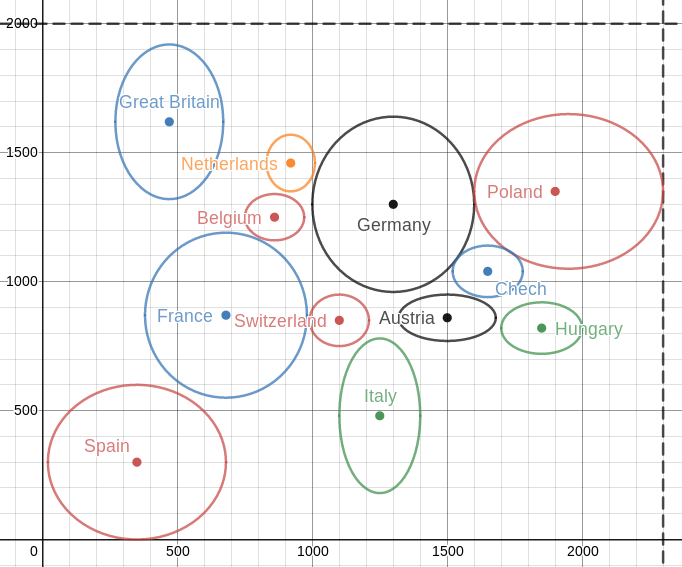
\includegraphics[width=\textwidth]{europe_coordinates}
        \caption{Europe}
        \label{fig:eur}
    \end{subfigure}
    \hfill
    \begin{subfigure}[b]{0.3\textwidth}
        \centering
        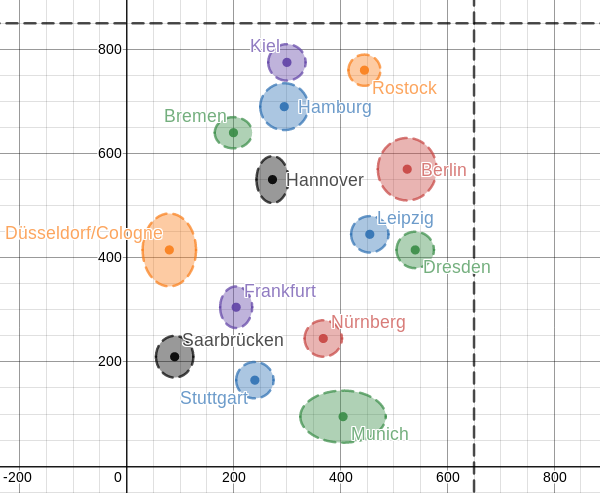
\includegraphics[width=\textwidth]{germany_coordinates}
        \caption{Germany}
        \label{fig:ger}
    \end{subfigure}
    \hfill
    \begin{subfigure}[b]{0.3\textwidth}
        \centering
        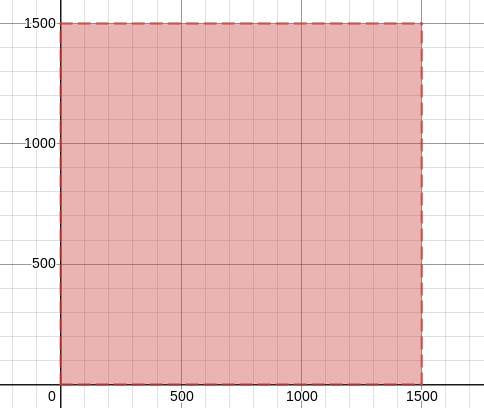
\includegraphics[width=\textwidth]{uniform_coordinates}
        \caption{Uniform}
        \label{fig:uni}
    \end{subfigure}
    \caption{Area of random point generation}
    \label{fig:areas}
\end{figure}

For the selected elipse a point was selected within the elipse at random with a uniform distribution.
For \fref{fig:uni} points were generated at random within the limits shown.
From our 5 instance sets, two were generated using \fref{fig:eur}, two with \fref{fig:ger} and one with the uniform distribution from \fref{fig:uni}. 
If a point belong in the same factory as a previously generated point, that point was generated within a reasonable radius of three kilometer.

\subsection{Generated Instances}
\label{sec:geni}
For testing our algorithm in this paper, 5 instance sets of each 5 instances of varying sizes were generated. Among the 5 instance sets, 2 were generated based on \fref{fig:eur}, two based on \fref{fig:ger} and one based on \fref{fig:uni}. Each instance set contains the following sizes:
TODO: Describe the instances I have generated and how I frefer to them in the paper. 
Finish the presentation of the results first to, know how I do this.

\section{Results}
\label{sec:res}
In the first two parts of this section we will present the data from our experiments, that leads to the final composition of our model. The results for the final algorithm are presented in the third part of this section.

\subsection{Evaluation of the wild algorithm}
\label{sec:evalw}
TODO: work on title of this section.
To help our algorithm out of a stuck position we designed a wild algorithm described in section \fref{sec:wild}. To evaluate the implementaion of this operator we have decided to evaluate the result of running the complete ALNS with all heuristics included with three different modifications. 
First we run the algorithm without any modification, also without the wild algorithm. 
Secondly we ran the algorithm including the wild algorithm. 
Lastly we ran the algorithm with a modification that resets the algorithm each time we get stuck and start from another starting point. 
The result from these three rund are summarized in \fref{fig:wildcomp}.

\subsection{Evaluation of heuristics}
\label{sec:evalh}
Different heuristics have different strengths and weaknesses. Some heuristics are not performing well on their own, but work very well in combination with other heuristics. 
Other heuristics are stron on their own, and their performance is prohibited by other heuristics, or not getting enough running time when too many heuristics are included.

\par To find the right combination of heuristics we have done an evaluation of their performance to search for the best possible combination of operators. To do this selected the instance set with a representative size of ... and ran our algorithm, without the wild algorithm adaptation, with each combination of operators.
This results in $2^7 = 128$ each running 10 times. To be able to compare the results from differnt instances we calculated the improvements from the initial solution which resulted in the improvement from the best solution found during the 10 runs, and an average improvement from the initial solution from the 10 runs of each combination.

\par We evaluated the data resulting from the different combination in three steps:
\begin{itemize}
    \item In the first part we ranked the combinations based on the best improvement and the average improvement
    \item In the second part we ran ANOVA and regression analysis to see which heuristics have a significant impact on the result
    \item In the third part we run t-tests to see if certain heuristics in combination with others have a positive or a negative impact on the final result
\end{itemize}

\subsubsection{Ranking the combinations}
We shorten the names of each heuristic and will refer to them for here on as components. The components are assigned the following names:
\begin{itemize}
    \item C1: this is the swap heuristic described in \fref{sec:swap}
    \item C2: exchange heuristic from \fref{sec:exch}
    \item C3: is the 2-opt heuristic in \fref{sec:2opt} 
\end{itemize}
\begin{figure}
    \centering
    \begin{subfigure}[b]{0.95\textwidth}
        \centering
        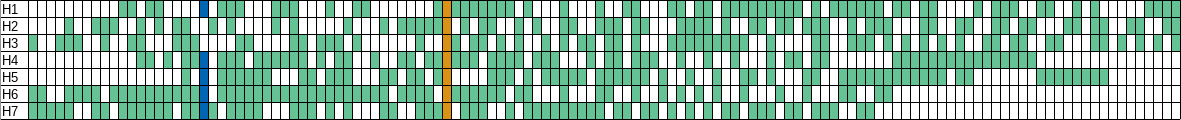
\includegraphics[width=\textwidth]{avrg_imp_rank}
        \caption{Average improvement}
        \label{fig:avrgrank}
    \end{subfigure}

    \begin{subfigure}[b]{0.95\textwidth}
        \centering
        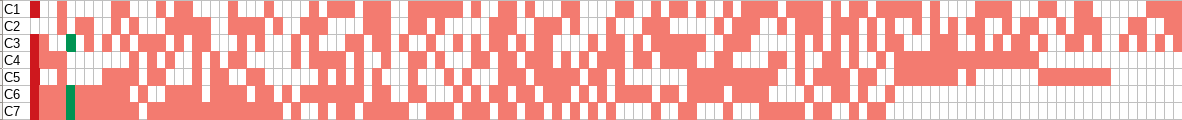
\includegraphics[width=\textwidth]{best_imp_rank}
        \caption{Best improvement}
        \label{fig:bestrank}
    \end{subfigure}

    \begin{subfigure}[b]{0.95\textwidth}
        \centering
        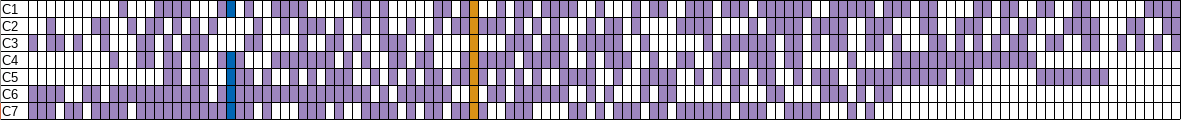
\includegraphics[width=\textwidth]{best_avrg_imp_rank}
        \caption{Best+Average improvement}
        \label{fig:avrgbestrank}
    \end{subfigure}
    \caption{Ranking of improvements from initial solution, the highlighted tiles indicate use of acomponent. Strongly highlighted combinations represent the best combination in one of the figures.}
    \label{fig:rank}
\end{figure}



\subsubsection{ANOVA and regression analysis}

\subsubsection{T-tests}

\subsection{Evaluation of algorithm}
\label{sec:evala}

\section{Observations}
\label{sec:obs}
This section will focus on the observation made from the results in the previous section.

\subsection{Choosing the final composition}
\label{sec:choosing}

\subsection{Performance of final composition}
\label{sec:fincomp}

\biblio                                                         
\end{document}  
